% Section 3: Results. Follows paper/outline.md, Section 3: one subsection per figure claim, Figures 2 to 6.
% Figure 1 (study design) belongs at the opening of Methods and is deliberately NOT placed here.
% Every result number is a \Num... macro from paper/numbers.tex (generated by paper/R/export_numbers.R).
\section{Results}\label{sec:results}

All results are simulated, ex ante and conditional on the explored ranges of the tool inputs, including zero to three years of cycle compression, which no study we found has measured and which the model applies as a scenario.

%==============================================================================
\subsection{Assumed Cycle Compression Separates Tool Profiles, and Accuracy Buys Months}\label{sec:res_time}

Years of cycle compression sort the annual genetic-gain uplift of the \NumNcellsOK\ simulated tool profiles into four groups, while measurement accuracy and plot cost spread profiles only within each group (Figure~\ref{fig:fig2_time_beats_accuracy}a). The separation follows from the model's arithmetic: one year of compression raises annual gain by \NumCycOneYearPct\% by construction, because the per-cycle gain is divided by a cycle of $L-1$ years instead of $L$. The median annual uplift over manual phenotyping was \NumAnnUpliftCycZero\% at zero compression and rose to \NumAnnUpliftCycOne\%, \NumAnnUpliftCycTwo\% and \NumAnnUpliftCycThree\% at one, two and three years. The interquartile ranges of the four groups (\NumAnnUpliftCycZeroQone\ to \NumAnnUpliftCycZeroQthree, \NumAnnUpliftCycOneQone\ to \NumAnnUpliftCycOneQthree, \NumAnnUpliftCycTwoQone\ to \NumAnnUpliftCycTwoQthree\ and \NumAnnUpliftCycThreeQone\ to \NumAnnUpliftCycThreeQthree\%) do not overlap, and the full ranges of adjacent groups overlap only in their tails. At zero compression, the uplift arises from accuracy and cost alone and averages \NumDGdiffPct\% per cycle across profiles.

\begin{figure}[H]
\begin{adjustwidth}{-\extralength}{0cm}
\centering
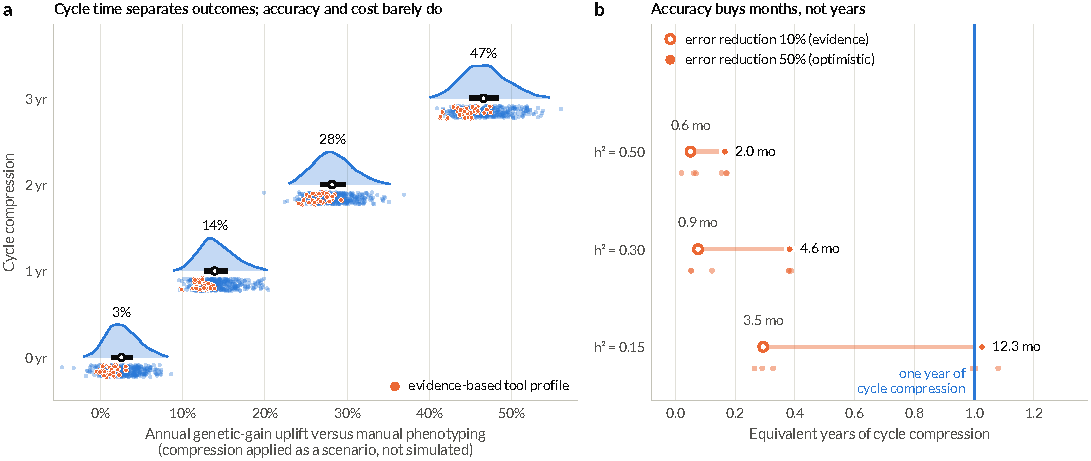
\includegraphics[width=\linewidth]{figures/fig2_time_beats_accuracy.pdf}
\end{adjustwidth}
\caption{Cycle time separates tool profiles, and accuracy buys months, not years. (\textbf{a}) Annual genetic-gain uplift over manual phenotyping across all simulated tool profiles, by years of cycle compression, which is applied as a scenario and not simulated (cloud: density; rain: profiles; bar and ring: interquartile range and median). Orange: evidence-based profile. (\textbf{b}) Exchange rate between accuracy and cycle time: years of breeding-cycle compression whose effect on annual genetic gain equals the tool's per-cycle uplift at the evidence-based and at the largest explored error reduction, by plot-level heritability (large markers: mean over the three on-station GxE parameter levels; small dots: individual settings). The uplift is averaged over the cost reductions of the robustness block and therefore includes their effect.\label{fig:fig2_time_beats_accuracy}}
\end{figure}

Accuracy gains within the range supported by the evidence are worth months, not years, of cycle compression (Figure~\ref{fig:fig2_time_beats_accuracy}b). In the robustness block, the per-cycle uplift at the evidence-based error reduction of \NumCfgErrRedCentral\% has the same effect on annual gain as \NumExchMoHtwoLowErrTen, \NumExchMoHtwoMidErrTen and \NumExchMoHtwoHighErrTen months of compression at the lowest, central and highest plot-level heritability (\NumCfgRobHtwoLow, \NumCfgHtwoYield\ and \NumCfgRobHtwoHigh). At the largest error reduction explored (\NumCfgErrRedMax\%), the equivalents are \NumExchMoHtwoLowErrFifty, \NumExchMoHtwoMidErrFifty and \NumExchMoHtwoHighErrFifty months. One full year of compression raises annual gain by \NumCycOneYearPct\%, a level that accuracy reaches only at the lowest heritability combined with the largest error reduction. Because the profiles that carry each error reduction also carry cost reductions, these equivalents overstate what accuracy alone buys.

The profile defined by the meta-analytic error and cost reductions draws almost all of its advantage from compression. This evidence-based profile (error reduction \NumCfgErrRedCentral\%, whole-plot cost reduction \NumCfgCostRedCentral\%) falls below the group median in every compression group (Figure~\ref{fig:fig2_time_beats_accuracy}a). Its median per-cycle uplift was \NumUpliftMeta\%, and its annual uplift was \NumAnnUpliftMetaCycZero\%, \NumAnnUpliftMetaCycOne\%, \NumAnnUpliftMetaCycTwo\% and \NumAnnUpliftMetaCycThree\% at zero to three years of compression.

%==============================================================================
\subsection{Accuracy and Cost Savings Move Per-Cycle Gain by a Few Percent}\label{sec:res_gain}

Per-cycle gain rises steadily with measurement-error reduction but stays below the annual-gain effect of one year of compression at the central heritability (Figure~\ref{fig:fig3_gain_ceiling}a). The mean paired per-cycle difference between the tool and the manual program rose from \NumDGdiffErrZero\ kg/ha at zero error reduction through \NumDGdiffErrTen, \NumDGdiffErrTwenty, \NumDGdiffErrThirty\ and \NumDGdiffErrForty\ kg/ha to \NumDGdiffErrFifty\ kg/ha at the largest reduction, against a manual gain of \NumDGtradPerCycle\ kg/ha per cycle (uncalibrated simulation units). In relative terms, the median uplift rose from \NumUpliftErrZero\% to \NumUpliftErrFifty\%, whereas one year of compression raises annual gain by \NumCycOneYearPct\%. Averaged over all profiles, the paired difference was \NumDGdiffPerCycle\ kg/ha (\NumDGdiffPct\% of the manual gain), with a mean Monte Carlo standard error of \NumDGdiffSE\ kg/ha. A negative mean difference occurred in \NumNcellsNegDiff\ of the \NumNcellsOK\ profiles, \NumNcellsNegDiffErrZero of them at zero error reduction. At zero error reduction the mean difference (\NumDGdiffErrZero\ kg/ha) is of the size of the standard error, so the sign of a single low-accuracy profile is partly Monte Carlo noise, and a tool fixed cost that neither accuracy nor cheaper plots offset can add to it.

\begin{figure}[H]
\centering
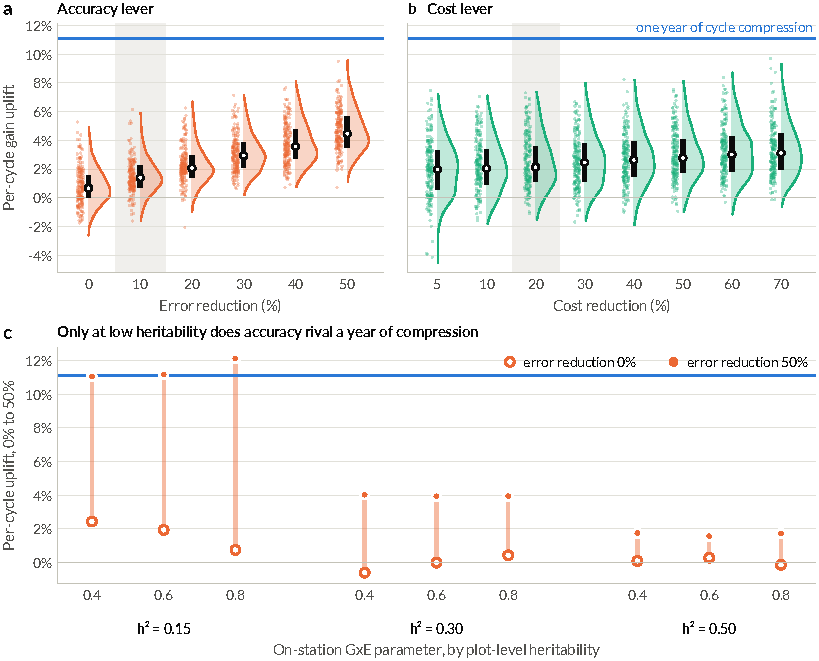
\includegraphics[width=\linewidth]{figures/fig3_gain_ceiling.pdf}
\caption{Accuracy and cost savings move per-cycle genetic gain by a few percent. (\textbf{a},\textbf{b}) Per-cycle genetic-gain uplift of the tool over manual phenotyping across all simulated tool profiles, by measurement-error reduction (\textbf{a}) and whole-plot cost reduction (\textbf{b}) ($h^2 = \NumCfgHtwoYield$; cloud: density; rain: profiles; bar and ring: interquartile range and median); shaded columns: evidence-based values. The vertical axes show the full range of the profiles, including negative uplifts. (\textbf{c}) Robustness: per-cycle uplift with no and with the largest error reduction for each combination of plot-level heritability and on-station GxE parameter. Blue lines: the annual-gain increase from one year of cycle compression.\label{fig:fig3_gain_ceiling}}
\end{figure}

Cheaper plots shift per-cycle uplift only modestly across their explored range (Figure~\ref{fig:fig3_gain_ceiling}b). Raising the whole-plot cost reduction from \NumCfgCostRedMin\% to \NumCfgCostRedMax\% moved the median per-cycle uplift from \NumUpliftCostFive\% to \NumUpliftCostSeventy\%. A fixed budget converts plot savings into more entries and environments, and selection gain shows diminishing returns to intensity and accuracy \cite{Cobb2019Enhancing}. The uplift was also larger at the smallest program budget (\NumUpliftBudgetLow\%) than at the largest (\NumUpliftBudgetHigh\%), a pattern consistent with a budget that limits trial size.

Only at the lowest plot-level heritability does the largest error reduction raise per-cycle gain to the level of one year of compression (Figure~\ref{fig:fig3_gain_ceiling}c). Averaged over the three GxE parameter levels, the per-cycle uplift at zero and at the largest error reduction was \NumRobUpliftHtwoLowErrZero\% and \NumRobUpliftHtwoLowErrFifty\% at the lowest heritability, \NumRobUpliftHtwoMidErrZero\% and \NumRobUpliftHtwoMidErrFifty\% at the central heritability, and \NumRobUpliftHtwoHighErrZero\% and \NumRobUpliftHtwoHighErrFifty\% at the highest. The one-year compression effect is \NumCycOneYearPct\%. At the central and highest heritability, the uplift stays well below that line at every GxE parameter level. Varying the on-station GxE parameter moved the uplift less than varying plot-level heritability did.

%==============================================================================
\subsection{Value Follows the Assumed Cycle Time}\label{sec:res_value}

The tool has a positive NPV in \NumPrNPVpos\% of the \NumNlookupRows\ profile-state combinations, and median NPV rises with each year of compression (Figure~\ref{fig:fig4_value_follows_time}a). Over all profiles and economic states, the median NPV was \NumNPVallCycZero million USD at zero compression and \NumNPVallCycThree million USD at three years. The evidence-based profile lay below the all-profile median at every compression level, at \NumNPVmetaCycZero and \NumNPVmetaCycThree million USD at zero and three years. Negative NPV occurred only at zero compression, and the number of negative values at one to three years was \NumNegNPVnonzeroComp.

\begin{figure}[H]
\begin{adjustwidth}{-\extralength}{0cm}
\centering
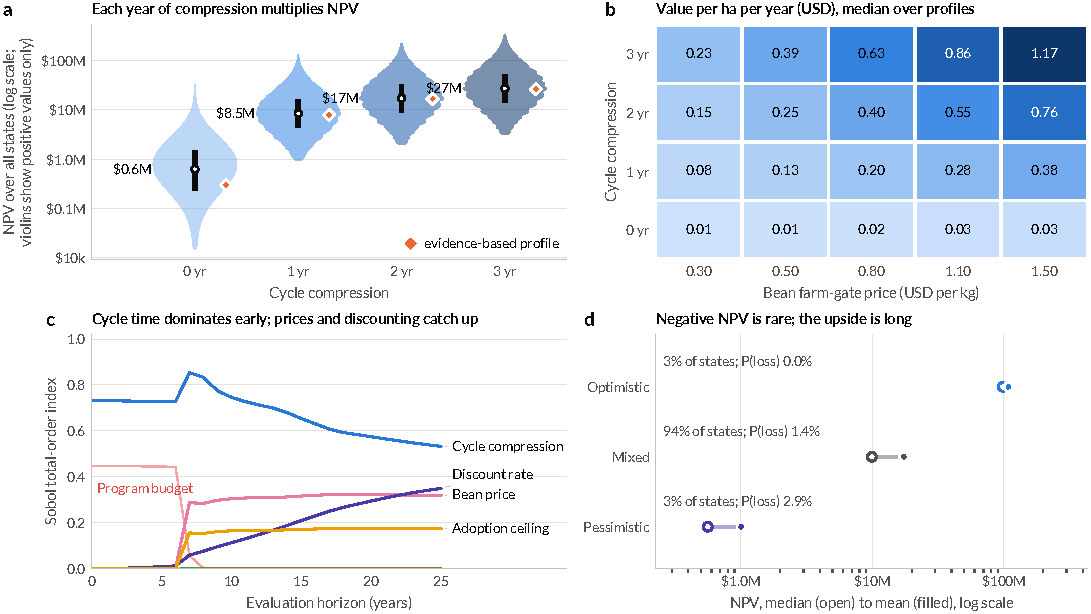
\includegraphics[width=\linewidth]{figures/fig4_value_follows_time.pdf}
\end{adjustwidth}
\caption{Value follows cycle time. (\textbf{a}) NPV of the tool across all tool profiles and economic states by cycle compression (violins of the positive values on a log scale; labels, bar and ring: median and interquartile range of all states; orange diamonds: median of the evidence-based profile). (\textbf{b}) Median equivalent annual value per hectare by cycle compression and bean price (discount rate \NumBaseDisc\%, adoption ceiling \NumBaseAdopt\%, bean area \NumBaseArea\ million ha). (\textbf{c}) Sobol total-order indices by evaluation horizon; the four inputs with the largest index at the final year and the program budget are labeled. (\textbf{d}) Median and mean NPV in the pessimistic and optimistic corners of the input space and in the remaining (mixed) states; P(loss): share of states with negative NPV.\label{fig:fig4_value_follows_time}}
\end{figure}

At the baseline economic state, the median equivalent annual value is small without compression and rises almost linearly with each year compressed (Figure~\ref{fig:fig4_value_follows_time}b). The baseline state has a bean price of \NumBasePrice\ USD/kg, a discount rate of \NumBaseDisc\%, an adoption ceiling of \NumBaseAdopt\% and a bean area of \NumBaseArea\ million ha. The median value was \NumEAAcycZero\ USD per hectare per year at zero compression and \NumEAAcycOne, \NumEAAcycTwo\ and \NumEAAcycThree\ USD per hectare per year at one, two and three years, or about \NumEAAperYearCompressed\ USD per hectare per year for each year compressed. The corresponding median NPV was \NumNPVcycZero, \NumNPVcycOne, \NumNPVcycTwo\ and \NumNPVcycThree\ million USD. NPV was positive in \NumPrPosCycZero\% of profiles at zero compression and in all profiles (\NumPrPosCycOne\%) at one, two and three years. Without compression, the value per hectare varied little across profiles (mean \NumConsEAAmean, standard deviation \NumConsEAAsd\ USD per hectare per year). Bean price raised the value within every row; at three years of compression, the median rose from \NumEAAcycThreePriceLow\ to \NumEAAcycThreePriceHigh\ USD per hectare per year between the lowest and highest price. These per-hectare values are small, and they become material only when summed over the \NumBaseArea\ million ha of the baseline state.

Median value stays positive in the most pessimistic economic state, and the dominance of compression is largest early in the horizon (Figure~\ref{fig:fig4_value_follows_time}c). In the state with the lowest price, highest discount rate, lowest adoption ceiling and smallest area (not shown in the figure), the median NPV across profiles was \NumStressMedianNPV\ million USD. For every tested pair of levels of two tool inputs, the median NPV over the remaining tool inputs in that state stayed positive (smallest value \NumStressMinMarginalNPV\ million USD). Before the first releases, NPV truncated at an evaluation year consists of incremental program costs, and it depends almost entirely on compression and program budget through the timing of spending. The total-order index of compression was \NumDynSTCycYearFive\ at year five, against \NumDynSTBudgetYearFive\ for program budget. It peaked at \NumDynSTCycPeak\ in year \NumDynSTCycPeakYear, the year of the earliest possible release, and declined to \NumDynSTCycFinal\ at year \NumCfgHorizon\ as discount rate, price and adoption ceiling gained weight.

Negative NPV is rare by construction, and the upside is concentrated in the optimistic corner (Figure~\ref{fig:fig4_value_follows_time}d). Both programs spend the same budget and tool costs replace plots within it, so NPV turns negative only where the simulated per-cycle gain difference is negative. The pessimistic corner (\NumScnPessimisticProb\% of states) had a mean NPV of \NumScnPessimisticMean\ and a median of \NumScnPessimisticMedian\ million USD, with \NumScnPessimisticPrNeg\% of states below zero. The mixed states (\NumScnOtherProb\%) had a mean of \NumScnOtherMean\ and a median of \NumScnOtherMedian\ million USD, with \NumScnOtherPrNeg\% below zero. The optimistic corner (\NumScnOptimisticProb\%) had a mean of \NumScnOptimisticMean\ and a median of \NumScnOptimisticMedian\ million USD, with \NumScnOptimisticPrNeg\% below zero. The mean exceeded the median in every group, which indicates right-skewed NPV distributions.

The main NPV excludes the cost of developing, hosting and supporting the tool. The median equivalent annual value multiplied by the area gives the level annual cost at which NPV falls to zero in the baseline state: \NumBECostCycZero, \NumBECostCycOne, \NumBECostCycTwo\ and \NumBECostCycThree\ million USD per year at zero to three years of compression. The only source we read on running cost puts a global AI phenotyping system at ``a few million USD per year'' \cite{Lasdun2024Participatory}, which exceeds the break-even cost at one year of compression and is of the same order as that at three years. Table~\ref{tab:netvalue} subtracts illustrative annual costs from the NPV. At \NumCfgRunCostLow\ million USD per year, the break-even compression was \NumBECompCostLow\ years, the expected net NPV was \NumRvEVCostLow\ million USD and it was positive in \NumRvPrPosCostLow\% of states. At \NumCfgRunCostHigh\ million USD per year, it was \NumRvEVCostHigh\ million USD and positive in \NumRvPrPosCostHigh\% of states, and the baseline-state median stayed negative at three years of compression (\NumRvNPVCycThreeCostHigh\ million USD).

\begin{table}[H]
\caption{Value of the tool net of an incremental running cost paid in every year of the horizon. Expected net NPV and the share of states with positive net NPV are over all tool profiles and economic states of the exact grid (bean area at the baseline). Break-even compression is the compression at which the median equivalent annual value at the baseline state, multiplied by the area, equals the running cost (linear interpolation between whole years). Median NPV is at the baseline economic state. EVPPI is at a decision hurdle of zero (invest or not).\label{tab:netvalue}}
\begin{adjustwidth}{-\extralength}{0cm}
\footnotesize
\setlength{\tabcolsep}{3pt}
\begin{tabularx}{\fulllength}{>{\raggedright\arraybackslash}X>{\centering\arraybackslash}p{1.4cm}>{\centering\arraybackslash}p{1.5cm}>{\centering\arraybackslash}p{1.6cm}>{\centering\arraybackslash}p{1.6cm}>{\centering\arraybackslash}p{1.6cm}>{\centering\arraybackslash}p{1.6cm}>{\centering\arraybackslash}p{1.4cm}>{\centering\arraybackslash}p{1.4cm}>{\centering\arraybackslash}p{1.5cm}}
\toprule
\textbf{Running cost (million USD per year)} & \textbf{Expected NPV} & \textbf{Share positive (\%)} & \textbf{Break-even compression (years)} & \textbf{Median NPV, 1 year} & \textbf{Median NPV, 3 years} & \textbf{EVPPI, compression} & \textbf{EVPPI, discount rate} & \textbf{EVPPI, price} & \textbf{EVPPI, error reduction}\\
\midrule
None (main analysis) & \NumRvEVBase & \NumRvPrPosBase & -- & \NumRvNPVCycOneBase & \NumRvNPVCycThreeBase & \NumEVPPIzeroHurdleMax & \NumEVPPIzeroHurdleMax & \NumEVPPIzeroHurdleMax & \NumEVPPIzeroHurdleMax\\
\NumCfgRunCostLow & \NumRvEVCostLow & \NumRvPrPosCostLow & \NumBECompCostLow & \NumRvNPVCycOneCostLow & \NumRvNPVCycThreeCostLow & \NumRvEVPPIzeroCycCostLow & \NumRvEVPPIzeroDiscCostLow & \NumRvEVPPIzeroPriceCostLow & \NumRvEVPPIzeroErrCostLow\\
\NumCfgRunCostMid & \NumRvEVCostMid & \NumRvPrPosCostMid & \NumBECompCostMid & \NumRvNPVCycOneCostMid & \NumRvNPVCycThreeCostMid & \NumRvEVPPIzeroCycCostMid & \NumRvEVPPIzeroDiscCostMid & \NumRvEVPPIzeroPriceCostMid & \NumRvEVPPIzeroErrCostMid\\
\NumCfgRunCostHigh & \NumRvEVCostHigh & \NumRvPrPosCostHigh & \NumBECompCostHigh & \NumRvNPVCycOneCostHigh & \NumRvNPVCycThreeCostHigh & \NumRvEVPPIzeroCycCostHigh & \NumRvEVPPIzeroDiscCostHigh & \NumRvEVPPIzeroPriceCostHigh & \NumRvEVPPIzeroErrCostHigh\\
\bottomrule
\end{tabularx}
\end{adjustwidth}
\end{table}

A tool noisier than manual scoring shows the downside that the main grid lacks. The stress block (error reduction \NumCfgStressErr\%, \NumNcellsStress\ profiles) changed per-cycle gain by \NumStressUpliftPct\% on average, with profiles between \NumStressDiffMin\% and \NumStressDiffMax\%, a pattern consistent with a lower cost per plot and a reallocated budget offsetting part of the added noise. At zero compression the median NPV was \NumStressNPVCycZero\ million USD, and NPV was positive in \NumStressPrPosCycZero\% of states. At one year of compression, the median NPV was \NumStressNPVCycOne\ million USD and positive in \NumStressPrPosCycOne\% of states, so the assumed time saving outweighed the added noise in this model.

%==============================================================================
\subsection{What a Pilot Should Measure}\label{sec:res_measure}

Cycle compression accounts for the largest share of NPV variance, followed by discount rate, price and adoption ceiling (Figure~\ref{fig:fig5_what_to_measure}a). The first-order and total-order Sobol indices were \NumSobolSoneCyc\ and \NumSobolSTCyc\ for compression, \NumSobolSoneDisc\ and \NumSobolSTDisc\ for discount rate, \NumSobolSonePrice\ and \NumSobolSTPrice\ for price, and \NumSobolSoneAdopt\ and \NumSobolSTAdopt\ for adoption ceiling. The total-order indices of the other four technical inputs (error reduction, cost reduction, program budget and tool fixed cost) were \NumSobolSTErrRed, \NumSobolSTCostRed, \NumSobolSTBudget\ and \NumSobolSTFixCost, respectively, so these inputs add almost nothing to NPV variance over the explored ranges \cite{Pianosi2016Sensitivity}. The indices are exact on the grid, and adding Layer 1 simulation noise of the size of the standard error of each profile's paired difference moved no total-order index by more than \NumSobolBootMaxShift. The first-order indices sum to \NumSobolSumSone\ and the total-order indices to \NumSobolSumST, so interactions carry the remainder of the variance, as expected for an NPV that multiplies gain, price, adoption and area.

\begin{figure}[H]
\centering
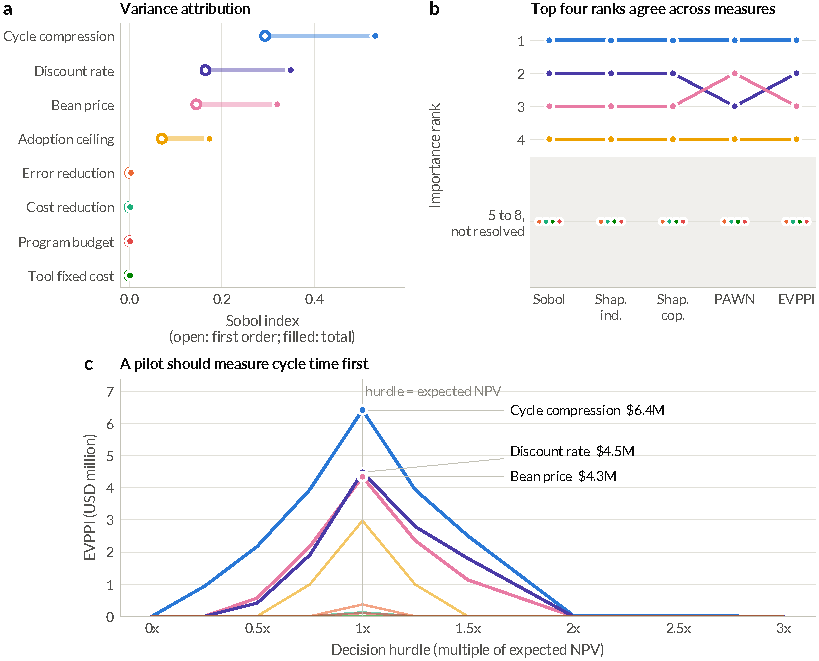
\includegraphics[width=\linewidth]{figures/fig5_what_to_measure.pdf}
\caption{What a pilot should measure. (\textbf{a}) First-order (open) and total-order (filled) Sobol indices of NPV. (\textbf{b}) Importance ranks of the inputs under five measures: Sobol total-order index, Shapley effects with independent and copula-correlated inputs, PAWN median, and EVPPI at the indifference hurdle; the four minor technical inputs (dots in the shaded band, colors as in panel a) lie below every other input on every measure, and their order is not resolved. (\textbf{c}) Expected value of perfect partial information (EVPPI) of each input as the payoff of the alternative investment varies (multiple of expected NPV); labels give the three largest values at the indifference point.\label{fig:fig5_what_to_measure}}
\end{figure}

When compression is fixed at zero, error reduction becomes the second-largest source of a much smaller NPV variance. The total-order indices were \NumSobolCycZeroSTDisc\ for discount rate, \NumSobolCycZeroSTErrRed\ for error reduction, \NumSobolCycZeroSTPrice\ for price, \NumSobolCycZeroSTBudget\ for program budget, \NumSobolCycZeroSTCostRed\ for cost reduction, \NumSobolCycZeroSTAdopt\ for adoption ceiling and \NumSobolCycZeroSTFixCost\ for tool fixed cost. Accuracy therefore matters for the residual value, which is small in absolute terms (Section~\ref{sec:res_value}). At the baseline economic state and zero compression, raising error reduction from zero to \NumCfgErrRedMax\% raised the median NPV from \NumRvNPVErrZero\ to \NumRvNPVErrFifty\ million USD, whereas one year of compression with no error reduction gave \NumRvNPVCycOneErrZero\ million USD.

Cycle compression ranks first under all five importance measures. Discount rate and price share ranks two and three, with their order depending on the measure, adoption ceiling ranks fourth on every measure, and the four minor technical inputs lie below all of them, with an order that is not resolved (Figure~\ref{fig:fig5_what_to_measure}b). Shapley effects with correlated inputs were \NumShapleyCyc\ for compression, \NumShapleyDisc\ for discount rate, \NumShapleyPrice\ for price, \NumShapleyAdopt\ for adoption ceiling, \NumShapleyErrRed\ for error reduction, \NumShapleyBudget\ for program budget, \NumShapleyCostRed\ for cost reduction and \NumShapleyFixCost\ for tool fixed cost. With independent inputs, the Shapley effects of compression, discount rate, price and adoption ceiling were \NumShapleyIndepCyc, \NumShapleyIndepDisc, \NumShapleyIndepPrice\ and \NumShapleyIndepAdopt, and those of error reduction and cost reduction were \NumShapleyIndepErrRed\ and \NumShapleyIndepCostRed. All \NumShapleyBracketN\ independent-input effects lie between the first-order and total-order indices of their input. PAWN gave \NumPawnCyc\ for compression, \NumPawnPrice\ for price, \NumPawnDisc\ for discount rate and \NumPawnAdopt\ for adoption ceiling, against \NumPawnErrRed, \NumPawnBudget, \NumPawnCostRed\ and \NumPawnFixCost\ for the four minor technical inputs. The first active-subspace direction of the lookup mapped to the nearest simulated profile carried \NumASshareOne\% of the mean squared gradient and the first two directions \NumAScumTwo\%. The first direction loads mainly on cycle compression (\NumASloadCycOne) and the second mainly on the economic inputs. Shapley effects sum to one, whereas the total-order Sobol indices sum to \NumSobolSumST, so rankings rather than magnitudes are compared across measures \cite{Iooss2019Shapley,Puy2020Sensitivity}.

The ranking survived every change we made to the assumptions that favor compression (Table~\ref{tab:robust}). In all \NumRvNscenarios\ scenarios, compression kept the first rank on the total-order index, with indices between \NumRvSTCycMin\ and \NumRvSTCycMax, against \NumRvSTErrMin\ to \NumRvSTErrMax\ for error reduction, and the smallest ratio of the two indices was \NumRvRatioMin. Restricting compression to zero or one year left the total-order index of compression at \NumRvSTCycPriorZeroOne\ against \NumRvSTErrPriorZeroOne\ for error reduction, and seasonal steps of zero, \NumCfgSeasonMid\ and one year gave \NumRvSTCycPriorSeason\ against \NumRvSTErrPriorSeason. Putting probability \NumCfgZeroMassB\ on no compression raised the index of compression to \NumRvSTCycPriorZeroHeavy. Removing the ramp, adding recurrent cycles, extending the horizon to \NumCfgHorizonLong\ years or slowing adoption changed the index between \NumRvSTCycHorizonForty\ and \NumRvSTCycRecurrent. The combination of no ramp, a slow rate and a long horizon with compression of zero or one year was the least favorable to compression, with indices of \NumRvSTCycConservativeZeroOne\ against \NumRvSTErrConservativeZeroOne. The calibration target changed expected NPV from \NumRvEVTargetQuarter\ million USD at \NumCfgTargetLow\% per year to \NumRvEVTargetOne\ million USD at \NumCfgTargetHigh\% per year, but it left the total-order indices of compression and error reduction unchanged to the printed precision.

\begin{table}[H]
\caption{Robustness of the attribution and decision results to the prior on cycle compression, the economic structure and the calibration target. Expected NPV (million USD) and total-order Sobol indices are over the exact grid with bean area at the baseline; EVPPI (million USD) is at the indifference hurdle, the expected NPV of each scenario.\label{tab:robust}}
\begin{adjustwidth}{-\extralength}{0cm}
\footnotesize
\setlength{\tabcolsep}{3pt}
\begin{tabularx}{\fulllength}{>{\raggedright\arraybackslash}X>{\centering\arraybackslash}p{2.0cm}>{\centering\arraybackslash}p{2.4cm}>{\centering\arraybackslash}p{2.4cm}>{\centering\arraybackslash}p{2.4cm}>{\centering\arraybackslash}p{2.4cm}}
\toprule
\textbf{Scenario} & \textbf{Expected NPV} & \textbf{Total index, compression} & \textbf{Total index, error reduction} & \textbf{EVPPI, compression} & \textbf{EVPPI, error reduction}\\
\midrule
\multicolumn{6}{l}{\textit{Prior on cycle compression}}\\
Equal weight on zero to three years (main analysis) & \NumRvEVBase & \NumRvSTCycBase & \NumRvSTErrBase & \NumRvEVPPICycBase & \NumRvEVPPIErrBase\\
Zero or one year, equal weight & \NumRvEVPriorZeroOne & \NumRvSTCycPriorZeroOne & \NumRvSTErrPriorZeroOne & \NumRvEVPPICycPriorZeroOne & \NumRvEVPPIErrPriorZeroOne\\
Zero, \NumCfgSeasonMid{} or one year (half-year steps) & \NumRvEVPriorSeason & \NumRvSTCycPriorSeason & \NumRvSTErrPriorSeason & \NumRvEVPPICycPriorSeason & \NumRvEVPPIErrPriorSeason\\
Zero with probability \NumCfgZeroMassA, one to three years share the rest & \NumRvEVPriorZeroMass & \NumRvSTCycPriorZeroMass & \NumRvSTErrPriorZeroMass & \NumRvEVPPICycPriorZeroMass & \NumRvEVPPIErrPriorZeroMass\\
Zero with probability \NumCfgZeroMassB, one year with the rest & \NumRvEVPriorZeroHeavy & \NumRvSTCycPriorZeroHeavy & \NumRvSTErrPriorZeroHeavy & \NumRvEVPPICycPriorZeroHeavy & \NumRvEVPPIErrPriorZeroHeavy\\
\midrule
\multicolumn{6}{l}{\textit{Economic structure}}\\
No ramp: full per-cycle gain from release & \NumRvEVRampStep & \NumRvSTCycRampStep & \NumRvSTErrRampStep & \NumRvEVPPICycRampStep & \NumRvEVPPIErrRampStep\\
Recurrent cycles with continued spending & \NumRvEVRecurrent & \NumRvSTCycRecurrent & \NumRvSTErrRecurrent & \NumRvEVPPICycRecurrent & \NumRvEVPPIErrRecurrent\\
Horizon of \NumCfgHorizonLong{} years & \NumRvEVHorizonForty & \NumRvSTCycHorizonForty & \NumRvSTErrHorizonForty & \NumRvEVPPICycHorizonForty & \NumRvEVPPIErrHorizonForty\\
Adoption rate \NumCfgKLow & \NumRvEVKTen & \NumRvSTCycKTen & \NumRvSTErrKTen & \NumRvEVPPICycKTen & \NumRvEVPPIErrKTen\\
Adoption rate \NumCfgKMid & \NumRvEVKFifteen & \NumRvSTCycKFifteen & \NumRvSTErrKFifteen & \NumRvEVPPICycKFifteen & \NumRvEVPPIErrKFifteen\\
No ramp, rate \NumCfgKLow, horizon \NumCfgHorizonLong{} years & \NumRvEVConservative & \NumRvSTCycConservative & \NumRvSTErrConservative & \NumRvEVPPICycConservative & \NumRvEVPPIErrConservative\\
The same, compression of zero or one year & \NumRvEVConservativeZeroOne & \NumRvSTCycConservativeZeroOne & \NumRvSTErrConservativeZeroOne & \NumRvEVPPICycConservativeZeroOne & \NumRvEVPPIErrConservativeZeroOne\\
\midrule
\multicolumn{6}{l}{\textit{Calibration target (percent of mean yield per year)}}\\
\NumCfgTargetLow & \NumRvEVTargetQuarter & \NumRvSTCycTargetQuarter & \NumRvSTErrTargetQuarter & \NumRvEVPPICycTargetQuarter & \NumRvEVPPIErrTargetQuarter\\
\NumCfgTargetHigh & \NumRvEVTargetOne & \NumRvSTCycTargetOne & \NumRvSTErrTargetOne & \NumRvEVPPICycTargetOne & \NumRvEVPPIErrTargetOne\\
\bottomrule
\end{tabularx}
\end{adjustwidth}
\end{table}

Resolving uncertainty about cycle compression is worth more than resolving any other input at every hurdle with a nonzero information value, and resolving error reduction or cost reduction is worth almost nothing (Figure~\ref{fig:fig5_what_to_measure}c). At the indifference hurdle, where the alternative pays the expected NPV of \NumEVprior\ million USD, the expected value of perfect partial information was \NumEVPPIIndiffCyc\ million USD for compression, \NumEVPPIIndiffDisc\ for discount rate, \NumEVPPIIndiffPrice\ for price and \NumEVPPIIndiffAdopt\ for adoption ceiling. It was \NumEVPPIIndiffErrRed\ million USD for error reduction, \NumEVPPIIndiffCostRed\ for cost reduction, \NumEVPPIIndiffBudget\ for program budget and \NumEVPPIIndiffFixCost\ for tool fixed cost. This hurdle is not tied to a named alternative investment, and EVPPI peaks there by construction. At a hurdle of zero, the decision to invest or not, EVPPI is \NumEVPPIzeroHurdleMax\ million USD for every input, because the expected NPV is positive at every level of every input. Under this model, which excludes the cost of the tool, no information a pilot could gather would change the decision to invest. The value of information falls to \NumEVPPItwoXCyc\ million USD for compression at twice the expected NPV. When an annual running cost makes the decision depend on the information (Table~\ref{tab:netvalue}), compression is again the most valuable input to resolve among those a pilot could measure, with EVPPI of \NumRvEVPPIzeroCycCostLow, \NumRvEVPPIzeroCycCostMid\ and \NumRvEVPPIzeroCycCostHigh\ million USD at \NumCfgRunCostLow, \NumCfgRunCostMid\ and \NumCfgRunCostHigh\ million USD per year, and error reduction remains at \NumRvEVPPIzeroErrCostHigh\ million USD. Discount rate and price describe the decision context rather than quantities a pilot can measure, so cycle compression is the highest-ranked input that a pilot could resolve.

%==============================================================================
\subsection{Evidence Behind the Inputs}\label{sec:res_evidence}

Common-bean breeding programs realized close to \NumGainTargetPct\% of mean yield per year, and image-based tools agreed with manual references on average but unevenly by trait (Figure~\ref{fig:fig6_evidence}a,b; Table~\ref{tab:meta}). The pooled realized gain over \NumMAoneK estimates from \NumMAoneKclus programs was \NumMAoneEst\% per year (95\% CI \NumMAoneCIlo to \NumMAoneCIhi; 95\% prediction interval \NumMAonePIlo to \NumMAonePIhi; $I^2$ = \NumMAoneItwo\%) \cite{Chiorato2010Genetic,deFaria2018Efficiency,Zeffa2020Genetic,Amongi2023Gain}. The lower confidence limit lies near zero. Sensitivity analyses gave pooled values from \NumMAoneSensLo to \NumMAoneSensHi\% per year, and leaving out one program at a time gave \NumMAoneLOOmin to \NumMAoneLOOmax\%. By trait, the pooled tool-manual correlation was \NumMAtwoHeight for plant height, \NumMAtwoCounts for counts and \NumMAtwoDisease for disease severity, the last with a confidence interval that includes zero. Pooled realized gain of maize and rice in Africa, kept as context, was \NumMAoneOther\% per year. Pooled correlations were \NumMAtwoLegume\ for legumes and \NumMAtwoNonLegume\ for non-legumes. Small-study tests gave no clear evidence of asymmetry (Egger-type $p$ = \NumMAtwoEggerP, rank test $p$ = \NumMAtwoRankP), although their power is low. Across all traits, the pooled correlation between tool and manual measurements was $r$ = \NumMAtwoR (95\% CI \NumMAtwoCIlo to \NumMAtwoCIhi; 95\% prediction interval \NumMAtwoPIlo to \NumMAtwoPIhi; $I^2$ = \NumMAtwoItwo\%) over \NumMAtwoK effects from \NumMAtwoKclus studies, and it was \NumMAtwoNoPre when preprints were excluded. It mixes traits, platforms and reference types and is descriptive. Smartphone measures of seed size agreed poorly with caliper measures in one preprint, where image area differed in scale and definition from the caliper values \cite{Gijare2026Assessing}.

\begin{table}[H]
\caption{Meta-analysis results used to set model inputs.\textsuperscript{a}\label{tab:meta}}
\begin{adjustwidth}{-\extralength}{0cm}
\footnotesize
\setlength{\tabcolsep}{3pt}
\begin{tabularx}{\fulllength}{>{\raggedright\arraybackslash}X>{\centering\arraybackslash}p{1.2cm}>{\centering\arraybackslash}p{1.3cm}>{\centering\arraybackslash}p{2.5cm}>{\centering\arraybackslash}p{2.5cm}>{\centering\arraybackslash}p{0.9cm}>{\raggedright\arraybackslash}p{2.7cm}}
\toprule
\textbf{Quantity} & \textbf{\emph{k}} & \textbf{Estimate} & \textbf{95\% CI} & \textbf{95\% PI} & \textbf{\emph{I}\textsuperscript{2} (\%)} & \textbf{Use in model}\\
\midrule
\multicolumn{7}{l}{\textit{MA1: realized genetic gain}}\\
Realized gain, common bean, three-level model (\% of mean yield per year) & 8 (4) & 0.51 & 0.00 to 1.01 & $-$0.74 to 1.75 & 87 & Calibration target\\
One estimate per program & 4 & 0.48 & $-$0.47 to 1.43 & $-$1.51 to 2.47 & 95 & Sensitivity\\
Embrapa mixed-model estimate in place of the direct estimate & 8 (4) & 0.36 & $-$0.06 to 0.79 & $-$0.61 to 1.33 & 79 & Sensitivity\\
Without IAC 1997 to 2007 & 7 (4) & 0.72 & 0.25 to 1.19 & $-$0.16 to 1.60 & 60 & Sensitivity\\
With one added estimate whose standard error is imputed (rule A) & 9 (5) & 0.90 & 0.03 to 1.78 & $-$1.29 to 3.10 & 96 & Sensitivity\\
Realized gain, maize and rice in Africa (context) & 4 & 1.12 & $-$0.25 to 2.49 & $-$1.80 to 4.04 & 95 & Context only\\
\midrule
\multicolumn{7}{l}{\textit{MA2: tool-manual agreement and implied error reduction}}\\
Tool-manual correlation, all traits (\emph{r}) & 19 (14) & 0.86 & 0.73 to 0.93 & $-$0.11 to 0.99 & 99 & Reported\\
Peer-reviewed studies only & 14 (10) & 0.89 & 0.79 to 0.94 & 0.29 to 0.99 & 98 & Sensitivity\\
Plant height & 4 & 0.95 & 0.77 to 0.99 & 0.00 to 1.00 & 100 & Subgroup\\
Plant count & 8 (4) & 0.85 & 0.69 to 0.93 & 0.26 to 0.98 & 88 & Subgroup\\
Disease severity & 3 & 0.68 & $-$0.29 to 0.96 & $-$0.89 to 1.00 & 98 & Subgroup\\
Manual-scoring reliability as entered (\emph{r}) & 3 & 0.90 & 0.56 to 0.98 & $-$0.17 to 1.00 & 92 & Used in T2 as entered\\
Manual-scoring validity after conversion (\emph{r}) & 3 & 0.95 & 0.76 to 0.99 & 0.22 to 1.00 & 92 & Used in T2 converted\\
Implied error reduction, reference error free, T1 (\%) & -- & $-$43 & $-$254 to 42\textsuperscript{b} & -- & -- & Evidence route\\
Implied error reduction, T2 with the reliability as entered (\%) & -- & 24 & $-$203 to 96\textsuperscript{b} & -- & -- & Evidence route\\
Implied error reduction, T2 with the converted validity (\%) & -- & $-$85 & $-$491 to 78\textsuperscript{b} & -- & -- & Evidence route\\
Implied error reduction, heritability pairs (\%) & 4 & 11 & $-$405 to 13\textsuperscript{b} & -- & -- & Central value (rounded)\\
\midrule
\multicolumn{7}{l}{\textit{MA3: time and cost savings}}\\
Time reduction, digital versus manual (\%) & 10 (7) & 95 & 87 to 98 & 7 to 100 & -- & Reported\\
Time reduction, handheld tools in field plots, capture time (\%) & 2 & 67 & 56 to 79\textsuperscript{b} & -- & -- & Cost reduction\\
Time reduction with the seed-counting null result added (\%) & 11 (7) & 93 & 81 to 97 & $-$101 to 100 & -- & Sensitivity\\
Share of plot cost that is not plot handling (\%) & 3 (1) & 30 & 25 to 36\textsuperscript{b} & -- & -- & Cost reduction\\
Implied whole-plot cost reduction, handheld tools (\%) & 6 & 20 & 14 to 29\textsuperscript{b} & -- & -- & Central cost reduction\\
\bottomrule
\end{tabularx}
\end{adjustwidth}
\noindent{\footnotesize{Estimates are pooled by restricted maximum likelihood; the interval for the Monte Carlo and descriptive rows is the 2.5 to 97.5 percentile range or the minimum to maximum, and the time reductions are unweighted because no study reports a variance. $k$: number of effects (number of programs or studies); CI: confidence interval; PI: prediction interval; $I^2$: heterogeneity. \textsuperscript{a} Included studies. MA1, common bean: \cite{Amongi2023Gain,Chiorato2010Genetic,deFaria2018Efficiency,Zeffa2020Genetic}; MA1, other crops: \cite{Asea2023Genetic,Menkir2022Estimating,Mukaro2024Genetic,Tarekegne2024Genetic,Todeschini2019Soybean,Yadav2026Genetic}; MA2: \cite{Banerjee2021Machine,FernandezGallego2018Wheat,Gijare2026Assessing,Guo2025Dlmlpc,Karisto2017Ranking,Liu2021Pocketmaize,Makanza2018Highthroughput,McDonald2022Automated,Mohammadi2024Enhancing,Parrella2013Evaluation,SadeghiTehran2019Deepcount,Volpato2023Digital,Zang2022Estimation,Zang2023Fieldmeasured}; MA3: \cite{DeBruin2025Breaking,Haghighattalab2016Application,Komyshev2017Evaluation,Mwanje2026Digital,Tanger2017Fieldbased,Walter2019Highthroughput,Zu2025Automated}. \textsuperscript{b} Descriptive: median with minimum to maximum, not pooled.}}
\end{table}


\begin{figure}[H]
\centering
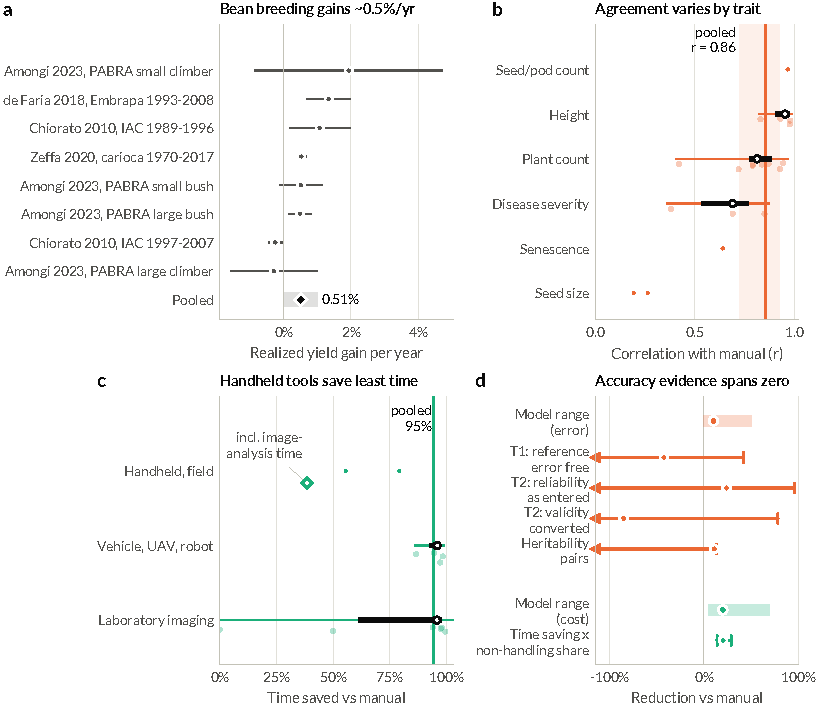
\includegraphics[width=\linewidth]{figures/fig6_evidence.pdf}
\caption{Evidence behind the model inputs. (\textbf{a}) Realized yield gain of common-bean breeding programs by program and period (dots and lines: estimates with 95\% intervals; diamond and band: three-level REML estimate and 95\% CI of the pool). IAC and Embrapa are Brazilian programs of the source studies. (\textbf{b}) Agreement between image-based or AI tools and manual reference measurements by trait (dots: individual effects; bar and ring: interquartile range and median for traits with several effects; line: pooled estimate; band: its 95\% CI). (\textbf{c}) Time saved by digital phenotyping relative to manual recording, by platform (dots: individual units; bar and ring: interquartile range and median where there are enough units; line: pooled estimate over all platforms). For handheld tools there are two descriptive units, and the open diamond is the capture-time saving of one of them when image-analysis time is counted. (\textbf{d}) Ranges of measurement-error and whole-plot cost reduction explored by the model (bars; dots: central case) against the evidence (points: median or estimate; lines: 95\% interval, or minimum to maximum for the heritability pairs; arrows: the interval continues beyond $-$115\%).\label{fig:fig6_evidence}}
\end{figure}

Digital tools save most data-capture time, handheld field tools save the least, and the implied error and cost reductions lie at the low end of the ranges the model explores (Figure~\ref{fig:fig6_evidence}c,d). Pooled over \NumMAthreeK units, digital tools reduced time per unit of data by \NumMAthreeTime\% (95\% CI \NumMAthreeTimeCIlo to \NumMAthreeTimeCIhi), a value dominated by mechanized platforms and laboratory imaging. For handheld tools in field plots, the estimates ranged from \NumMAthreeHandheldLo to \NumMAthreeHandheldHi\% (descriptive only; \NumMAthreeHandheldK units, the upper value derived from times reported for a smartphone field workflow) \cite{Walter2019Highthroughput,Lasdun2024Participatory}. When image-analysis time is counted, the capture-time saving of the lower unit fell to \NumMAthreeWalterTotal\% \cite{Walter2019Highthroughput}. A study of smartphone grain counting found no time saving \cite{Komyshev2017Evaluation}. Multiplying the share of plot cost that is not plot handling \cite{Reynolds2019Costefficient} by the field handheld time saving implies a whole-plot cost reduction of \NumMAthreeCostRed\% (range \NumMAthreeCostRedLo\ to \NumMAthreeCostRedHi\%), which is an upper bound on the saving from data capture alone.

The tool-manual correlation does not identify error reduction, because it depends on how reliable the manual reference is. The manual-reliability evidence from three studies pooled to \NumMAtwoManualRel\ (95\% CI \NumMAtwoManualRelLo\ to \NumMAtwoManualRelHi) when every coefficient was entered as a correlation with the true value. That pool mixes correlations of raters with a digital measure of the truth, correlations between two raters, and squared correlations, and the study with the first kind alone gave \NumMAtwoManualTruthOnly. After converting each coefficient to a correlation with the true value, the pooled validity of manual scoring was \NumMAtwoManualRelV\ (95\% CI \NumMAtwoManualRelVLo\ to \NumMAtwoManualRelVHi), which exceeds, although its interval includes, the break-even value of \NumMAtwoBreakEvenRel\ at which a tool correlated \NumMAtwoR\ with manual scores would equal manual scoring. The implied error reduction had a median of \NumERtOne\% when the manual reference is treated as error free (95\% interval \NumERintTOneLo\ to \NumERintTOneHi\%), \NumERtTwo\% when it carries the pooled manual error as entered (\NumERintTTwoLo\ to \NumERintTTwoHi\%), \NumERtTwoV\% after the conversion (\NumERintTTwoVLo\ to \NumERintTTwoVHi\%), and \NumERhtwoMedian\% from heritability pairs (range \NumERintHtwoLo\ to \NumERintHtwoHi\%). The heritability pairs set the central value of the model. Route T1 and the converted route T2 give negative medians, route T2 as entered gives a positive one but rests on the pool that mixes coefficient types, and the probability of a positive error reduction was \NumERprTOnePos\%, \NumERprTTwoPos\% and \NumERprTTwoVPos\% for the three correlation-based routes. The intervals or ranges of all four routes include zero improvement.
